\chapter{About Dresden OCL}
\label{chapter:about}

\begin{flushright}
\textit{Chapter written by Claas Wilke and Michael Thiele}
\end{flushright}

\emph{Dresden OCL} is developed as a project at the Technische Universit�t 
Dresden (TUD), Software Technology Group since 1999. Its latest version is 
released as a set of Eclipse plug-ins and thus, is sometimes also referred
as \emph{\acl{DOT4Eclipse}}. Dresden OCL consists of a set of OCL tools,
including an OCL parser, an OCL interpreter, an OCL-to-Java and an OCL-to-SQL
code generator.

In this chapter, some general information on Dresden OCL is presented. The 
supported OCL version and the differences to the official OCL specification are 
documented. Supported meta-models, models and model instances are shortly
presented. If you are not interested in such information, you can skip this 
chapter and continue with the installation and general use of Dresden OCL as 
documented in Chapter~\ref{chapter:introduction}.
  


\section{Supported Version of OCL}

Dresden OCL generally supports \oclversion as specified in~\cite{spec:OCL2-3}. 
Nevertheless, some differences between Dresden OCL and \oclversion exist as
documented in the following:


\subsection{Comformance of Dresden OCL to the \oclversion specification}

The \oclversion specification defines a set of compliance points that can be
addressed by tools implementing OCL~\cite[p.~1]{spec:OCL2-3}.
Table~\ref{tab:compliance} summarises the compliance points addressed by
Dresden OCL.

\begin{table}[h]
\begin{tabular}{|p{7cm}|p{7cm}|}
    \hline
    \textbf{Compliance Point} & \textbf{Support in Dresden OCL} \\
    \hline
    Syntax & 
    Fully supported (Except \code{OclMessage}, its related operations, and
    \code{OclAny.oclLocale()}).
    \\
    \hline
    XMI & 
    XMI export/import of OCL is currently not supported. \\
    \hline
    Evaluation & 
    \\
    - \code{allInstances()} &
    supported \footnotesize(with some limitations to specific
    technological spaces, e.g., Java) \\
    - \code{@pre} in postconditions &
    supported \\
    - \code{OclMessage} & 
    not supported \\
    - Navigating non-navigable association ends & 
    not supported \\
    - accessing private and protected features & 
    supported \\
    \hline
\end{tabular}
\caption{Compliance points addressed by Dresden OCL (v. 3.x) according
to~\cite[p.~1]{spec:OCL2-3}.}
\label{tab:compliance}
\end{table}

Besides the features enlisted in Table~\ref{tab:compliance} some minor
differences exist between Dresden OCL and the OCL specification:

\begin{itemize}
  \item Dresden OCL does not support the operation \texttt{OclAny.oclLocale()}
  introduced within \oclversion that can be used to implement different behavior for
  the \texttt{String} operations \texttt{to\-Low\-er\-Case()},
  	\texttt{to\-Upper\-Case()}, \texttt{<(String)}, \texttt{>(String)},
  	\texttt{<=(String)}, and \texttt{>=(String)}.
  	Since Dresden OCL is implemented in Java, it uses the semantics of
  	\texttt{java.lang.String.to\-Low\-er\-Case()},
  	\texttt{to\-Upper\-Case()}, and
  	\texttt{compareTo(String)} instead.
  \item Dresden OCL does not support the expression of
  	UnlimitedNaturalExpressions to define multiplicities within constraints such
  	as \texttt{(1..*)}.
\end{itemize}
	
	
\subsection{Different Semantics of OCL Expressions in Dresden OCL}

The current \oclversion specification~\cite{spec:OCL2-3} contains some
inconsistencies and misses some definitions especially when evaluating
\code{invalid} or \code{null} values. Thus, we had to assume or change the
semantics of OCL during evaluation of some OCL statements. In the following
we present the differences of the OCL semantics used in Dresden OCL compared 
with the official OCL specification~\cite{spec:OCL2-3}.


\subsubsection{Boolean Operators}

\begin{table}
	\centering
		\begin{tabular}{|p{1.2cm}p{1.2cm}||p{1.2cm}|p{1.2cm}|p{1.2cm}|p{1.2cm}|p{2.0cm}|}
			\hline
      \textbf{a}	& \textbf{b}	& \textbf{not a}	& \textbf{a or b}	& \textbf{a xor b} 	& \textbf{a and b}	& \textbf{a implies b} \\
			\hline
			false				&	false				&	true						&	false						& false							&	false							&	true \\
			\hline	
			false				&	true				&	- `` -						&	true						& true							&	false							&
			true
			\\
			\hline
			false				&	null				&	- `` -							&	invalid					& invalid						&	false							&	true \\
			\hline
			false				&	invalid			&	- `` -							&	invalid					& invalid						&	false							&	true \\
			\hline
			true				&	false				&	false						&	true						& true							&	false							&	false \\
			\hline
			true				&	true				&	- `` -							&	true						& false							&	true							&	true \\
			\hline
			true				&	null				&	- `` -							&	true						& invalid						&	invalid						&	invalid \\
			\hline
			true				&	invalid			&	- `` -							&	true						& invalid						&	invalid						&	invalid \\
			\hline
			null				&	false				&	invalid					&	invalid					& invalid						&	false							&	invalid \\
			\hline
			null				&	true				&	- `` -							&	true						& invalid						&	invalid						&
			true \\
			\hline
			null				&	null				&	- `` -							&	invalid					& invalid						&	invalid						&	invalid \\
			\hline
			null				& invalid			&	- `` -							&	invalid					& invalid						&	invalid						&	invalid \\
			\hline
			invalid			& false				&	invalid					&	invalid					& invalid						&	false							&	invalid \\
			\hline
			invalid			&	true				&	- `` -							&	true						& invalid						&	invalid					
			&	true \\
			\hline
			invalid			&	null				&	- `` -							&	invalid					& invalid						&	invalid						&	invalid \\
			\hline
			invalid			&	invalid			&	- `` -							&	invalid					& invalid						& invalid						&	invalid \\
			\hline
		\end{tabular}
		\caption{Decision Table for boolean operators in Dresden OCL.}
		\label{tab:decisionTable}
\end{table}

Boolean operators in Dresden OCL are interpreted as documented in 
Table~\ref{tab:decisionTable}. As documented, the operator \code{and} always 
results in \code{false} as long as one of its operands is \code{false}, ignoring
whether the other operand is \code{null} or even \code{invalid}. The operator 
\code{or} results in \code{true}, as long as one of its operands is \code{true}.
Both \code{false implies null} and \code{false implies invalid} result in 
\code{true}. The operator \code{xor} can only be evaluated if both arguments 
are neither \code{null} nor \code{invalid}. Otherwise the operand will result in
\code{invalid}.


\subsubsection{Equality in Dresden OCL}

\begin{table}
	\centering
		\begin{tabular}{|p{1.2cm}p{1.2cm}||p{1.2cm}|p{1.2cm}|p{1.2cm}|p{1.2cm}|p{1.2cm}|p{1.2cm}|}
			\hline
      \textbf{a} 	& \textbf{b} 	& \textbf{a = b} 	& \textbf{a <> b} 	& \textbf{a < b} 	& \textbf{a <= b} 	& \textbf{a > b} 	& \textbf{a >= b} \\
			\hline
			42					&	42					&	true						&	false							&	false						&	true							&	false							&	true \\
			\hline
			42					&	7						&	false						&	true							&	false						&	false							&	true							&	true \\
			\hline
			42					&	null				&	false						&	true							&	invalid					&	invalid						&	invalid						&	invalid \\
			\hline
			null				&	null				&	true						&	false							&	invalid					&	invalid						&	invalid						&	invalid \\
			\hline
			42					&	invalid			&	false						&	true							&	invalid					&	invalid						&	invalid						&	invalid \\
			\hline
			invalid			&	invalid			&	true						&	false							&	invalid					&	invalid						&	invalid						&	invalid \\
			\hline
		\end{tabular}
		\caption{Decision Table for equality operators in Dresden OCL.}
		\label{tab:info:equalityDecisionTable}
\end{table}

\acs{OCL} defines the two operators \code{=} and \code{<>} to compute equality 
of two given \acs{OCL} expressions. Since \acs{OCL} values can be both
\code{null} or \code{invalid}, it is important to know how these operators 
behave when used with \code{null} and \code{invalid} values. According to the 
specification, comparing two \acs{OCL} values results in \code{invalid} when 
one of the two values is either \code{null} or
\code{invalid}~\cite[p.~214]{spec:OCL2-3}. In some situations this can lead to
problems during evaluation, e.g., when iterating on an \acs{OCL} collection 
containing \code{null} values.

Thus in Dresden OCL, using the operators \code{=} and \code{<>} for comparison
will always result in \code{true} or \code{false} as documented in 
Table~\ref{tab:info:equalityDecisionTable}. But please be aware, that this 
behaviour is only implemented for \code{=} and \code{<>}. Using other comparison
operators such as \code{<}, \code{<=}, \code{>}, and \code{>=} for numeric 
values can result in \code{invalid}!


\subsubsection{Collections}

In Dresden OCL, collections can contain \code{null} values but cannot contain 
\code{invalid} values! If an \code{invalid} value is contained in a collection, 
the complete collection will be \code{invalid} as well.


\subsubsection{Iterators}

\begin{figure}[t]
\lstset{keywords={Bag, true, false, invalid, null}, label={lst:exampleIterators}, caption={Some example Iterator Expressions and their evaluation results.}, captionpos=b}
\begin{lstlisting}
Bag { true, null } -> exists(true) => true
Bag { true, null } -> forAll(true) => invalid
Bag { true, null } -> one(true) => true
Bag { true, null } -> one(false) => invalid
Bag { true, null } -> select(true) => invalid
Bag { true, null } -> select(oclIsUndefined()) => Bag { null }
\end{lstlisting}
\end{figure}

In Dresden OCL, iterators will result in a value as long as they can be computed,
even if their collection contains \code{null} values. 
Listing~\ref{lst:exampleIterators} shows some examples for iterator expressions 
and their results in Dresden OCL (e.g., an \code{any} iterator will result in 
\code{true} as long as one element of its source's collection fulfills its 
condition even if other elements are \code{null} values). On the other hand, a 
\code{select} iterator will result in \code{invalid} if the condition for any 
element in its collection results in \code{null}. However, if the collection 
contains \code{null} values but the condition results in \code{true} or 
\code{false} (e.g., \code{oclIsUndefined()}), the result will not be 
\code{invalid}.

A further difference between the \acs{OCL} specification and the semantics in
Dresden \acs{OCL} exists for the \texttt{closure()} iterator. According to the
specification, the \texttt{closure()} iterator computes its result based on a
depth-first search~\cite[Sect.~7.6.5]{spec:OCL2-3}, whereas results in Dresden
\acs{OCL} are computed based on breadth-first search, due to performance reasons.


\subsubsection{Handling of Null values}

\begin{figure}[t]
\lstset{keywords={Bag, true, false, invalid, null}, label={lst:info:nullValues}, caption={Evaluation of null values in Dresden OCL.}, captionpos=b}
\begin{lstlisting}
null + 2 => invalid
null.asSet() => Set { }
null.oclIsUndefined() => true
invalid.oclIsUndefined() => invalid
\end{lstlisting}
\end{figure}

According to the \oclversion specification~\cite{spec:OCL2-3}, all operation calls
invoked on \code{null} values will result in \code{invalid}. An exception is the
operation \code{oclIsUndefined()} which results in \code{true} if its source is 
\code{null} and \code{false} otherwise. According to the \oclversion specification 
the expression \code{invalid.oclIsUndefined()} will result in \code{true} as
well. \textbf{In Dresden OCL, \code{invalid.ocl\-Is\-Undefined()} results in 
\code{invalid} instead!} According to the \oclversion specification, the implicit 
OCL operation \code{asSet()} can be invoked on \code{null} values and will
result in an empty \code{Set}. Listing~\ref{lst:info:nullValues} shows some
examples for evaluations on \code{null} values.


\subsubsection{Handling of Invalid values}

\begin{figure}[t]
\lstset{keywords={Bag, true, false, invalid, null}, label={lst:info:invalidValues}, caption={Evaluation of invalid values in Dresden OCL.}, captionpos=b}
\begin{lstlisting}
invalid + 2 => invalid
invalid.asSet() => invalid
invalid.oclIsInvalid() => true
undefined.oclIsInvalid() => false
\end{lstlisting}
\end{figure}

According to the \oclversion specification~\cite{spec:OCL2-3}, all operation calls 
invoked on \code{invalid} values will result in \code{invalid}. Exceptions are 
the operations \code{oclIsInvalid()} and \code{oclIsUndefined()}. The evaluation
of \code{oclIsInvalid()} will result in \code{true} when invoked on 
\code{invalid} values. Otherwise it will result in \code{false}, even when 
invoked on \code{null} values. \code{invalid.asSet()} will result in 
\code{invalid} because sets cannot contain invalid values. 
Listing~\ref{lst:info:invalidValues} shows some examples for evaluations on 
\code{invalid} values.



\section{Supported Models In Dresden OCL}
\label{sect:info:models}

Dresden OCL is adapted to multiple metamodels and thus allows the import of 
multiple kinds of models. Which kinds of models and which model file formats are
supported by Dresden OCL is documented in this section. Possible use cases for
the different models and model instances supported by Dresden \acs{OCL} are
given in Section~\ref{sec:usecases}.


\subsection{EMF Ecore Models}

Dresden OCL allows to import Ecore models modelled with the
\emph{\acf{EMF}}~\cite{WWW:EMF}. Typically, Ecore models are stored in \acs{XMI}
files matching to the naming pattern \code{*.ecore}.


\subsection{Java Classes as Models}
\label{subsec:javaModel}

Dresden OCL supports to import Java classes as models and thus, to define
\acs{OCL} constraints directly on Java types and their fields and methods. If a 
Java class is imported into Dresden OCL, all types used inside the class' 
declaration are handled as also being a part of the imported model. If a 
\code{ClassA} is imported into Dresden OCL containing an attribute of the type 
\code{ClassB}, \code{ClassB} is also imported into Dresden OCL. \code{ClassB} 
could contain an operation having the return type \code{ClassC} and thus 
\code{ClassC} could be imported as well. After short consideration it should be 
clear that such a transitive mechanism could lead to a more or less complete
import of the Java standard library into Dresden OCL. Thus, only the types that 
are used during OCL parsing and evaluation are imported into Dresden OCL.

\begin{figure}[t]
\lstset{language=Java, label={lst:javaModelProvider}, caption={Example for a Java Model Provider Class.}, captionpos=b}
\begin{lstlisting}
package org.dresdenocl.examples.simple;

public class ModelProviderClass {

  protected Person person;

  protected Professor professor;

  protected Student student;
}
\end{lstlisting}
\end{figure}

If a \code{ClassA} is imported into Dresden OCL, the type of \code{ClassA} and
all types that are directly related to this class are imported as well (e.g., a 
\code{ClassB} used in a property of \code{ClassA} would be imported, a related 
\code{ClassC} used in \code{ClassB} would not be imported, see 
Figure~\ref{fig:info:transitiveTypeImport}). If other types are requested during
the work of tools on the imported model (e.g., if a tool requests the operation 
\code{ClassB.getOwnedOperations()}), all newly required types will be imported
as well. This deferred transitive adaptation mechanism avoids that all types never 
used inside Dresden OCL are imported and adapted and cause overhead and
maintenance problems. Listing~\ref{lst:javaModelProvider} shows an example for a
Java class provided with the \emph{Simple Example} of Dresden OCL. The class
contains properties having the types \code{Person}, \code{Professor} and 
\code{Student}. Thus, the imported model in Dresden OCL will contain a package 
\code{org.dresdenocl.example.simple}, containing the four classes 
\code{ModelProviderClass}, \code{Person}, \code{Professor} and \code{Student}.

\begin{figure}[t]
	\centering
		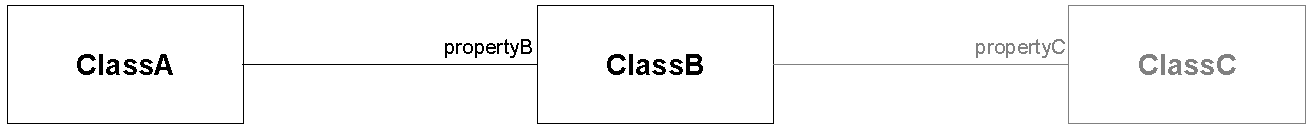
\includegraphics[width=1.00\textwidth]{figures/info/transitiveTypeImport.pdf}
	\caption{Transitive Import of Java Classes as a Model into Dresden OCL.}
	\label{fig:info:transitiveTypeImport}
\end{figure}

To import Java classes into Dresden OCL two possibilities exist:

\begin{enumerate}
	\item \code{*.class} files can be imported as a model. All directly referenced 
	  classes (either as types of properties and operations or their arguments) are
	  imported as well. \textbf{Please be aware, that only byte code classes
	  (\code{*.class}) and not source code classes \code{*.java} can be imported
	  into Dresden OCL!} However, the graphical, Eclipse-based version supports
	  selecting \code{*.java} files instead. In most cases the byte code resolving
	  should work correctly. If you intend using Dresden OCL without the provided
	  UI, you have to select \code{*.class} files instead.
	\item Alternatively, the path leading to the Java class to be imported can be 
	  declared in a text file matching to the file naming pattern
	  \code{*.javamodel}. This alternative was implemented to support the import of
	  Java classes referencing other external Java classes provided as \acs{JAR}s.
	  An example for a \code{*.javamodel} text file is shown in 
	  Listing~\ref{lst:javaModel}. The first line references the 
	  \code{JarClassProvider.class} that shall be imported as a model. The second 
	  line references a \acs{JAR} file that contains classes whose types are 
	  referenced in the \code{JarClassProvider.class}. Both, the class and the 
	  \acs{JAR} are referenced via relative \acs{URL}s from the directory where the
	  \code{*.javamodel} file is located in the file system. Further lines of the 
	  \code{*.javamodel} text file could be used to reference additional \acs{JAR}s
	  to be imported as well. Please be aware, that only referenced classes from 
	  the \acs{JAR}s are imported into Dresden OCL. Again, further classes are 
	  imported when required during \acs{OCL} parsing or evaluation.
\end{enumerate}

\begin{figure}[t]
\lstset{language=OCL, label={lst:javaModel}, caption={Example for a .javamodel File.}, captionpos=b}
\begin{lstlisting}
../bin/package1/package2/JarClassProvider.class
../lib/simple.jar
\end{lstlisting}
\end{figure}


\subsection{MDT UML Class Diagrams}

Dresden OCL allows to import UML class diagrams modelled with the 
\emph{\acf{Eclipse MDT}}~\cite{WWW:MDT}. Typically, \acs{MDT} \acs{UML} models
are stored as \acs{XMI} files matching to the naming pattern \code{*.uml}. 
Since many Eclipse-based modelling tools built on top of \acs{MDT} \acs{UML}, 
their models can be imported as well. Examples for such modelling tools are the 
\emph{\acf{GMF}} \acs{UML} class diagram editor and the \emph{Topcased}
\acs{UML} class diagram editor.


\subsection{XML Schemas as Models}

Dresden OCL allows to import \acl{XSD}s (\acs{XSD}) as models. Typically, 
\acs{XSD}s are stored in \acs{XML} files matching to the naming pattern 
\code{*.xsd}.



\section{Supported Model Instances In Dresden OCL}
\label{sect:info:modelinstances}

Dresden OCL is adapted to and thus, allows the import of multiple types of model 
instances. Which types of model instances are supported by Dresden OCL is 
documented in this section. Possible use cases for
the different models and model instances supported by Dresden \acs{OCL} are
given in Section~\ref{sec:usecases}.


\subsection{EMF Ecore-Based Model Instances}

Besides the creation of meta-models or \acs{DSL}s, the \acf{EMF} allows the 
generation of simple model editors that can be used to model instances of the 
Ecore-based models created before. E.g., you can create a simple \acs{DSL} 
using \acs{EMF}. Afterwards, you can model an instance of this \acs{DSL} using 
an Ecore-generated model editor. Now, you can import your \acs{DSL} as a model 
into Dresden OCL and you can parse \acs{OCL} constraints defined on your
\acs{DSL}. To check these constraints on the created model instance, you have to
import this instance into Dresden OCL as well.

Thus, Dresden OCL allows to import instances of Ecore-based models as model
instances. Typically, the instances are stored as \acs{XMI} files that match to
a file naming pattern that ends with the name of your Ecore model. E.g., if you 
modelled an \code{myDSL.ecore} and created an instance of this model via an 
Ecore-generated model editor, the instance matches to the naming pattern 
\code{*.mydsl}.

Besides complete models it can be useful to import single model instance
elements into Dres\-den OCL when using Dresden OCL directly from another
software application via its \acs{API}. How this is possible is documented in 
Section~\ref{sect:modelInstanceTypeAdaptation:addIMIElement}. For Ecore model 
instances, this mechanism can be used to add single \code{EObjects} to a model 
instance in Dresden OCL.


\subsection{Java Model Instances}
\label{subsec:javaInstance}

Java objects can be regarded as instances of model elements described in class 
diagrams or similar models. Thus, the import of Java objects as model instances 
for \acs{OCL} constraint interpretation is a common use case. Dresden OCL 
supports two possibilities to import Java objects into Dresden OCL.

\begin{figure}[t]
\lstset{language=Java, label={lst:info:javaModelInstance}, caption={Example for a ModelInstanceProviderClass programmed in Java.}, captionpos=b}
\begin{lstlisting}
public class ModelInstanceProviderClass {

  /**
   * @return A {@link List} of {@link Object}s that are part of the
   *         {@link IModelInstance}.
   */
  public static List<Object> getModelObjects() {

    List<Object> result;
    result = new ArrayList<Object>();

    Person person1;
    person1 = new Person();
    person1.setName("Person Unspecific");
    person1.setAge(25);
    result.add(person1);

    /* Add further elements ... */
		
    return result;
  }
}
\end{lstlisting}
\end{figure}

\begin{enumerate}
	\item It is possible to create a \code{ModelInstanceProviderClass} containing
	  a static method called \code{getModelObjects()} that returns a \code{List} of
	  \code{java.lang.Objects} that shall be imported as a model instance.
	  Listing~\ref{lst:info:javaModelInstance} shows an example of such a
	  \code{ModelInstanceProviderClass}.
	\item Similar to Ecore model instances, it is possible to add single 
	  \code{java.lang.Object}s to an existing model instance via Dresden OCL's
	  \acs{API} at runtime as documented in
	  Section~\ref{sect:modelInstanceTypeAdaptation:addIMIElement}.
\end{enumerate}


\subsection{XML Model Instances}

Dresden OCL supports to import \acs{XML} files as model instances. Although
\acs{XML} files cannot contain executable code, their elements can be used as
data to be verified by structural \acs{OCL} integrity constraints. Typically, 
\acs{XML} files conform to the file name matching pattern \code{*.xml}.



\section{Summary}

This chapter documented which version of OCL is supported by Dresden OCL. 
Furthermore, supported types of models and model instances were presented. The
following chapter will explain how to install and use Dresden OCL.
